\startchapter{The Large Hadron Collider and the ATLAS Experiment}
\label{chapter:lhcatlas}

The \textbf{Large Hadron Collider (LHC)} is the world's largest and most energetic proton-proton collider. It forms a 27 km circular ring beneath Switzerland and France, with its origin at the \textbf{Conseil Européen pour Recherche Nucléaire (CERN)} in Geneva. It began operation in 2008, and since then has collided over $10^{15}$ particles. The collider houses four major experiments: ALICE, ATLAS, CMS, and LHCb, along with several smaller projects. ALICE (A Large Ion Collider Experiment) studies heavy ion collisions, while LHCb (Large Hardon Collider beauty) specializes in studying the physics of the bottom quark. \textbf{ATLAS (A Toroidal LHC ApparatuS)} and CMS (Compact Muon Solenoid) are both general purpose experiments designed to study a wide range of interactions resulting from high-energy proton-proton collisions. This work uses data collected by the ATLAS experiment, and a description of the LHC accelerator and ATLAS detector follow in Sections \ref{section:lhc} and \ref{section:atlas} respectively.

\section{The Large Hadron Collider}
\label{section:lhc}
Built between 1998 and 2008, the LHC began colliding protons in 2010 at a center-of-mass energy of 7 TeV, and today most recently in 2018 collisions occured at 13 TeV. Successfully colliding particles at this energy is an immense technical challenge which is achieved by the many technologies of the LHC and its accelerator complex.

In order to reach a beam energy of 6.5 TeV, protons are slowly stepped up through a chain of accelerators before reaching the LHC. They begin their journey as hydrogen atoms, stripped of their electrons before beign accelerated to an energy of 50 MeV by the Linac2 linear accelerator. Following this the Proton Synchrotron Booster (PSB) accelerates them to 1.4 GeV, passing them to the Proton Synchrotron (PS) and then the Super Proton Synchrotron to be accelerated to 25 and then 450 GeV. Finally, beams are split into clockwise and counterclockwise directions and injected into the LHC where they are accelerated to theiir final 6.5 TeV energy.

The acceleration of the protons is achieved by radio-frequency cavities. These cavities contain a resonant electro-magnetic field oscillating at 400 MHz, which is applied to particles passing through. The LHC contains 8 cavities per beam, with each providing a maximum of 2 MV of potential, so each proton can recieve up to 16 MeV of energy per lap. As a result it takes millons of laps over a period of around 20 minutes for a proton injected at 450 GeV to reach its collision energy of 6.5 TeV.  These RF cavities also serve to keep each beam in bunches of $1.15 \times 10^{11}$ protons spaced at intervals of just 25 ns.

The crown jewel of LHC technology is its magnets. 1,232 superconducting NbTi dipole magnets kept at 1.9 K, each spanning 14.3 m and weighinh 35 tonnes, create an 8.3 Tesla magnetic. This field lies perpendicular to the beam path, bending it to its desired route. The bending dipole magnets are complemented by 392 quadrupole magnets that focus the beams to a small aperture, and many higher-order multipole magnets which provide small beam corrections.

Allong with the collisional energy of the accelerated particles, the other most important measure of a particle acceletator is the luminosity it achieves. \textbf{Luminosity ($\mathcal{L}$)} is used to determine the rate ($R$) at which a given interaction occurs using:

$$R = \mathcal{L}\sigma$$

where $\sigma$ is the cross-section of the desired interaction. As a result, when searching for rare processes, a obtaining a high luminosity is crucial.

The integrated luminosity, $L$, gives the total number of interactions over a period of time, and is defined as:

$$ L = \int \mathcal{L}\, dt$$

At the LHC, the luminosity is controlled by the number of bunches circulating $n_b$, the frequency of revolution $f_r$, $N_{1,2}$ the number of particles in each colliding bunch, and the cross sectional area of the colliding beams. This results in the equation:

$$\mathcal{L}  = \frac{ f_rn_bN_1N_2 }{4\pi\sigma_x\sigma_y}R_{\phi} $$

where $R_{\phi}$ is a geometrical loss factor caused by the beams crossing at an angle, and $\sigma_{x,y}$ are the horizontal and vertical widths of the beams, which are estimated to have a Gaussian profile. The LHC currently has a nominal peak luminosity of $\mathcal{L} = 10^{34} cm^{-2}s^{-1}$.

\section{The ATLAS Experiment}
\label{section:atlas}

The ATLAS experiment uses the LHC in combination with the general-purpose ATLAS detector to test a broad range of SM and BSM predictions. Together with the CMS experiment, its greatest achievement to date was the detection and discovery of the SM Higgs boson in 2012 \cite{HiggsDiscovery}.

\begin{figure}[H]
    \centering
    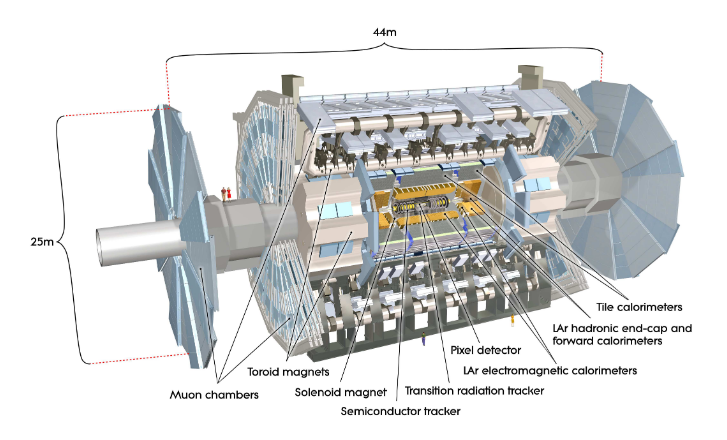
\includegraphics[width=0.8\textwidth]{Figures/2/ATLASDetector.png}
    \caption{A cut-out overview of the ATLAS detector and main components.}
    \label{fig:atlasdec}
\end{figure}

The ATLAS detector, an overview of which is shown in Figure \ref{fig:atlasdec}, is comprised of several layers, which work in tandem to detect many diverse particles. From inner-most to outer-most the layers are:

\begin{itemize}
    \item The inner detector, with excellent angular resolution to track charged particles.
    \item The electromagnetic calorimeters, designed primarily to measure the energy and position of electrons and photons.
    \item The hadronic calorimeters designed to measure the energy and position of hadrons.
    \item The muon spectrometer, to track and measure muons.
\end{itemize}

When combined with the electronics required to read and trigger on measurements, the entire detector weighs over 7000 t and measures 44 m long by 25 m wide and high. Its barreled shape with end caps covers nearly the full solid angle. The following sections will describe the layout and operations of the ATLAS detector in more detail.

\subsection{Inner Tracking Detector}
The ATLAS inner detector tracks the direction and momentum of charged particles immediately after leaving the interaction point. A 2 T superconducting solenoid surrounds the inner detector, bending charged particles with the Lorentz force, allowing their momentum to be determined from the curvature of their path. Within the inner detector, there are three separate sub-detectors: the pixel detector, the semiconductor tracker (SCT), and the transition radiation tracker (TRT). A cutout view of the detector is shown in Figure \ref{fig:atlasinner}.

\begin{figure}[H]
    \centering
    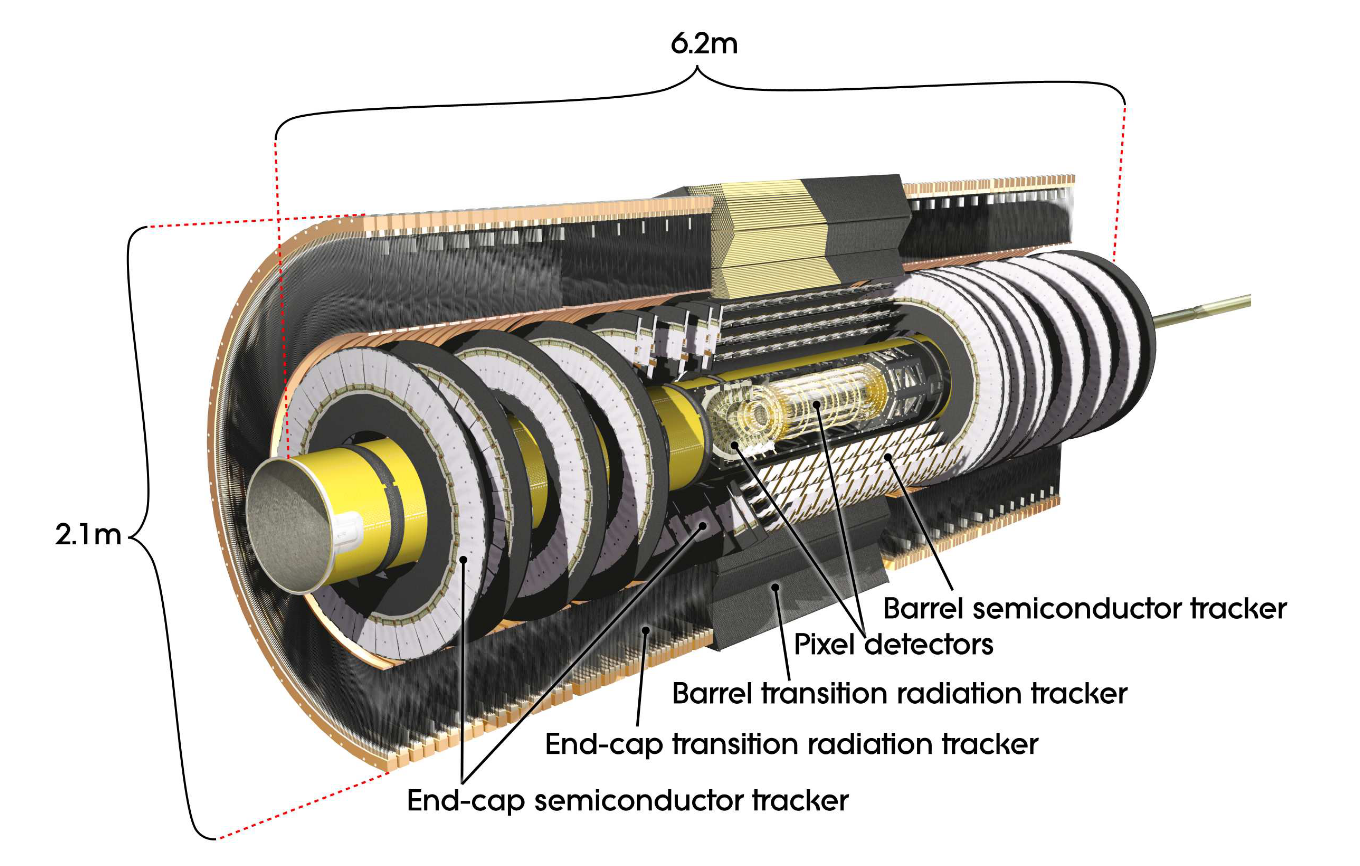
\includegraphics[width=0.8\textwidth]{Figures/2/InnerDetector.png}
    \caption{A cut-out view of the ATLAS inner detector.}
    \label{fig:atlasinner}
\end{figure}

The pixel detector consists of an array of 1744 pixel sensors, each containing 47232 silicon pixels, mostly measuring 50x400 $\mu m^2$. They are arranged into three cyclindrical layers and three disk-shaped layers on each end. The high granularity of these detectors ensures strong angular resolution, providing prescise measurements of vertex location and track momentum. Notably, this detector must be very radiation-hard in order to maintain performace over the detector lifespan in an area that recieves an immense radiation dose from the high particle flux.

Though it would be desireable, it would not be feasible to extend the high-resolution pixel detector because of the high cost and signal readout volume. As a result, in the SCT the point-like pixels are extended into silicon strip detectors, which are laid in pairs at an angle of 40 mrad to each other to allow measurements in two dimensions. The SCT is made up of four concentric cylindrical layers in the barrel and two disk-shaped layers on each end-cap.

The TRT is the final component of the component of the inner detector.  It consists of approximately 300000 drift tubes filled with majority Xenon gas, with the walls kept at -1.5 kV and a central wire at ground. When particles pass through the tubes, the gas is ionized and the resulting electrons drift to the centre where the signal is amplified. Additionally, the gaps between TRT straws are filled with polymer fibres (in the barrel) or foils (in the end caps). As a result, highly relativistic particles create transition radiation at the material interfaces, which aids with electron identification.


\subsection{Calorimeters}
The calorimeters
\subsection{Muon Spectrometers}
The muon detectors
\subsection{Trigger and Data Acquisition}
The trigger and DAQ
